\documentclass[10pt]{article}
\usepackage{amsfonts}
\usepackage{amsthm}
\usepackage{amssymb}
\usepackage{amsmath}
\usepackage{graphicx}
\usepackage{subcaption}
\usepackage{xcolor}
\usepackage{mathtools}
\usepackage{ wasysym }
\usepackage{enumerate}
\usepackage{verbatim}
\usepackage{hyperref}


\numberwithin{equation}{section}
\newcommand{\new}[2]{
    \vspace{2mm}
    \noindent
    \textbf{
    \underline{#1}}
    \textit{{#2}}
    \
}

\def\<{{\langle}}
\def\>{{\rangle}}

\DeclarePairedDelimiter\bra{\langle}{\rvert}
\DeclarePairedDelimiter\ket{\lvert}{\rangle}
\DeclarePairedDelimiterX\braket[2]{\langle}{\rangle}{#1\,\delimsize\vert\,\mathopen{}#2}


\newcommand{\textOr}{
    {
        \hspace{5mm}
        \textrm{or}
        \hspace{5mm}
    }
}

\newcommand{\textAnd}{
    {
        \hspace{5mm}
        \textrm{and}
        \hspace{5mm}
    }
}


\newcommand{\textWhere}{
    {
        \hspace{5mm}
        \textrm{where}
        \hspace{5mm}
    }
}



\newcommand{\Ixp}[1]{
    {
        e^{i{#1}}
    }
}



\newcommand{\halfFigure}[1]{
\begin{center}
\includegraphics[width = .5\linewidth]{{#1}}
\end{center}
}

\newcommand{\fullFigure}[1]{
\begin{center}
\includegraphics[width = .9\linewidth]{{#1}}
\end{center}
}

\def\twobytwoMat(#1, #2, #3, #4){
    {
        \begin{bmatrix}
            {#1} & {#2}\\
            {#3} & {#4}
        \end{bmatrix}
    }
}

\def\twobyoneMat(#1, #2){
    {
        \begin{bmatrix}
            {#1}\\
            {#2}
        \end{bmatrix}
    }
}

\def\twobytwoDet(#1, #2, #3, #4){
    {
        \begin{vmatrix}
            {#1} & {#2}\\
            {#3} & {#4}
        \end{vmatrix}
    }
}


\newcommand{\deriv}[2]{
\frac {d {#1} } {d {#2}}
}

\newcommand{\pderiv}[2]{
\frac {\partial {#1} } {\partial {#2}}
}


\newcommand{\RR}{\mathbb{R}}
\newcommand{\CC}{\mathbb{C}}
\newcommand{\ZZ}{\mathbb{Z}}
\newcommand{\Zpos}{\mathbb{Z}_{pos}}
\newcommand{\NN}{\mathbb{N}}

\newtheorem{theorem}{Theorem}
\newtheorem{proposition}{Proposition}
\newtheorem{lemma}{Lemma}
\newtheorem{corollary}{Corollary}
\newtheorem{remark}{Remark}
\newtheorem{definition}{Definition}
\newtheorem{example}{Example}
\newtheorem{conjecture}{Conjecture}
\newtheorem{question}{Question}

\numberwithin{theorem}{section}
\numberwithin{proposition}{section}
\numberwithin{lemma}{section}
\numberwithin{corollary}{section}
\numberwithin{remark}{section}
\numberwithin{definition}{section}
\numberwithin{example}{section}
\numberwithin{conjecture}{section}
\numberwithin{question}{section}



\newcommand{\ch}{\text{ch}}



\title{Quantized Oscillations Lab Report}
\author{Daeyoung Son}
\date{December 2024}

\begin{document}

\maketitle



\section{Setup and Methods}

\begin{figure}[htp]
    \centering
    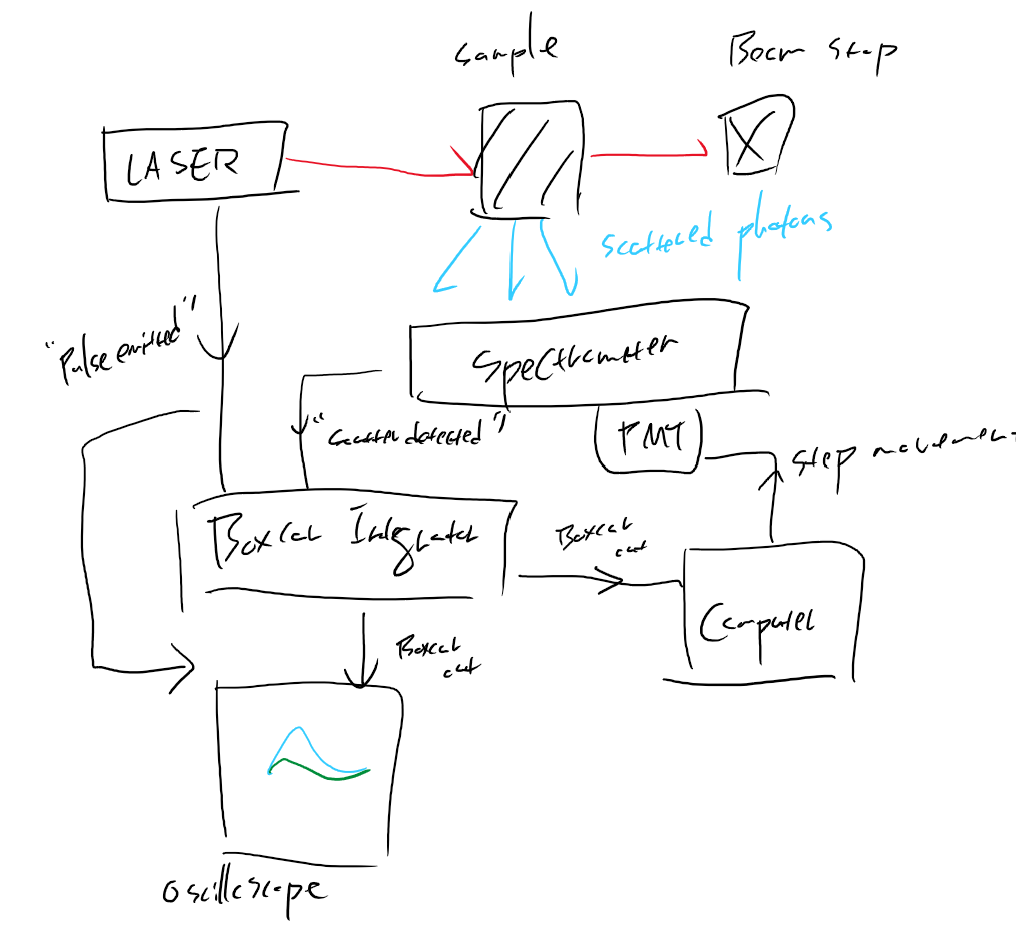
\includegraphics[width=0.8\textwidth]{setupFig.png} % Replace 'figure.jpg' with your image file
    \caption{Figure of the setup}
    \label{fig:example}
\end{figure}


    In this lab, we observe the interactions between 
    photons and molecules. When a photon collides a molecule, 
    the molecule is exciteted to a virtual state. Then, as the 
    molecule exits the virtual state and collapses to one of the 
    stable energy states it emits a photon. This process of 
    photon emission related to change of a molecule's vibrational mode 
    is called \textbf{Raman Scattering}. 

\subsection{General Setup}

Pulses of Nitrogen lazers are shot at the sample. As Raman Scattering 
occurs within the sample, the sample emits photons. These photons are 
emitted towards the spectrometer. A computer system drives the PMT 
motor in order to collect the emission around diverse range of spectra. 

Since the laser is emitted in form of pulses, it is imperitive to 
take measurements exactly at the point of the time when the pulse is emitted. 
In order to guarantee that the collected data has the hightest intensity 
originating from the pulse, we use the \textbf{Boxcar Integrator}. 

The Boxcar integrater accepts two inputs. The first is the signal input, 
and the second is the gate input. The gate input triggers the Boxcar 
integrator to set up a square pulse after a event. Then, the boxcar 
integrates the product of the generated square pulse and the signal 
input. The integrated value is proportional to the average sequence 
intensity in a short time period after the trigger. 

The Spectrometer consists of two slits. Narrowing down the 
distance between the slits guarantee better resolution of the data. 
However, as the slit is narrowed, less photons enter the detector, and 
a greater gain is required to amp up the spectrometer output signal. 

\subsection{Week 1: Vibrational Modes of Water and Benzene}

We explore the vibrational modes 
of Water($H_2O$) and Benzene ($C_6H_6$). 
The former has three vibrational modes and the latter 
has 30. Around the vibrational modes, 
we expect to observe a peak of measured intensity. 


\subsection{Week 2: Dye lasers and the Iodine molecule}

The molecules observed in week 1 have a complicated 
structure. We explore a simpler moleclue, Iodine($I_2$). 
The potential of this molecule can be losely considered 
as a simple harmonic oscillator. Since the energy eigenstates 
of a harmonic oscillator potential have equal spacings, 
we expect the measured intensity peaks to be equidistant for the 
iodine molecule. 

\section{Overview of Vibrational Peaks}

We first demonstrate the advantages of Raman Spectroscopy. 
The two close vibrational modes of the water molecule are at 
$3650 cm^{-1}$ and $3750 cm^{-1}$ which correspond to symmetric and 
asymmetric stretch. Suppose we wish to induce a vibrational mode 
change using classical absorbtion tecnhiques. The required wavelength 
of the driver photon can be computed by considering the energy difference 
between the two modes. 

\begin{align}
    \Delta E & = \ \Delta k \hbar c \ = \ \frac c {\lambda} \\ 
    \lambda & = \ \frac 1 {\Delta k} \ = \ \frac 1 {100 cm^{-1}} \ = \ 10^{-4} m
\end{align}

Such lambda in the magnitude of $-4$ is in the borderline of IR rays 
and radars. Therefore, it is impossible to drive a water molecule using 
a $N^2$ laser that has a wavelength of $\lambda_N = 535nm$. 

Raman Spectroscopy drives the molecule to a virtual energy state 
that is unstable. From the unstable state, the molecule might either 
fall to a higher or a lower energy eigenstate that it used to be. 
If after the scattering, the molecule gains energy, the wavelength shift in the incident 
and emitted photon is called \textbf{Stokes Shift}. If the molecule 
loses energy, the phenomenon is called a \textbf{anti-Stokes Shift}. 
In the perspective of the photon, the stokes shift are red since the 
photon loses energy. On the contrary, anti-stokes shifts are blue. 
The peaks in spectrum induced by these shifts are called \textbf{
    Stokes and anti-Stokes peaks
} or \textbf{Raman peaks}. 

If the temperature of the system is low, then most of the molecules 
will be in the lowest vibrational mode. If a photon is scattered 
upon a low-temperature sample, the molecule will always take energy 
from the photon, resulting in a stokes shift. Therefore, all 
the Raman peaks will be red. 

The distribution of molecules over the vibrational modes can 
be characterized by the boltzman distribution. The measured 
intensity corresponds to the population of the molecule. The 
intensity ratio can be quantified theoretically as follows. 

\begin{align}
    \frac {I} {I_{gr}} \ = \ \exp\left(
        -\frac {\Delta E}{k_B T}
    \right)
\end{align}

Here, $\Delta E$ corresponds to the energy difference between 
the vibrational mode in question and the ground state. 

\begin{question}
    At what temperature will a blue Raman peak will occur 
    in a $1/e$ intensity of the largest red Raman peak?
\end{question}

\begin{proof}[Solution]
    If we assume that the probability of occurence 
    of the stokes shifts are proportional to the population 
    density of molecules in each vibrational mode, 
    we can compute the temperature where 
    a change in energy between the 
    two peaks leads the argument of the 
    boltzman exponential to evaluate to $-1$. 
    At the desired temperature $T$, in Kelvins, 
    \begin{align}
        \frac {\Delta E}{k_B T} 
        \ = \ \frac{\Delta k \hbar c}{k_B T}\ = \ 1 \\ 
        T \ = \ \frac {(\Delta k) \hbar c}{k_B } \ = \ \boxed{469.7 K}
    \end{align}
\end{proof}

\begin{figure}[htp]
    \centering
    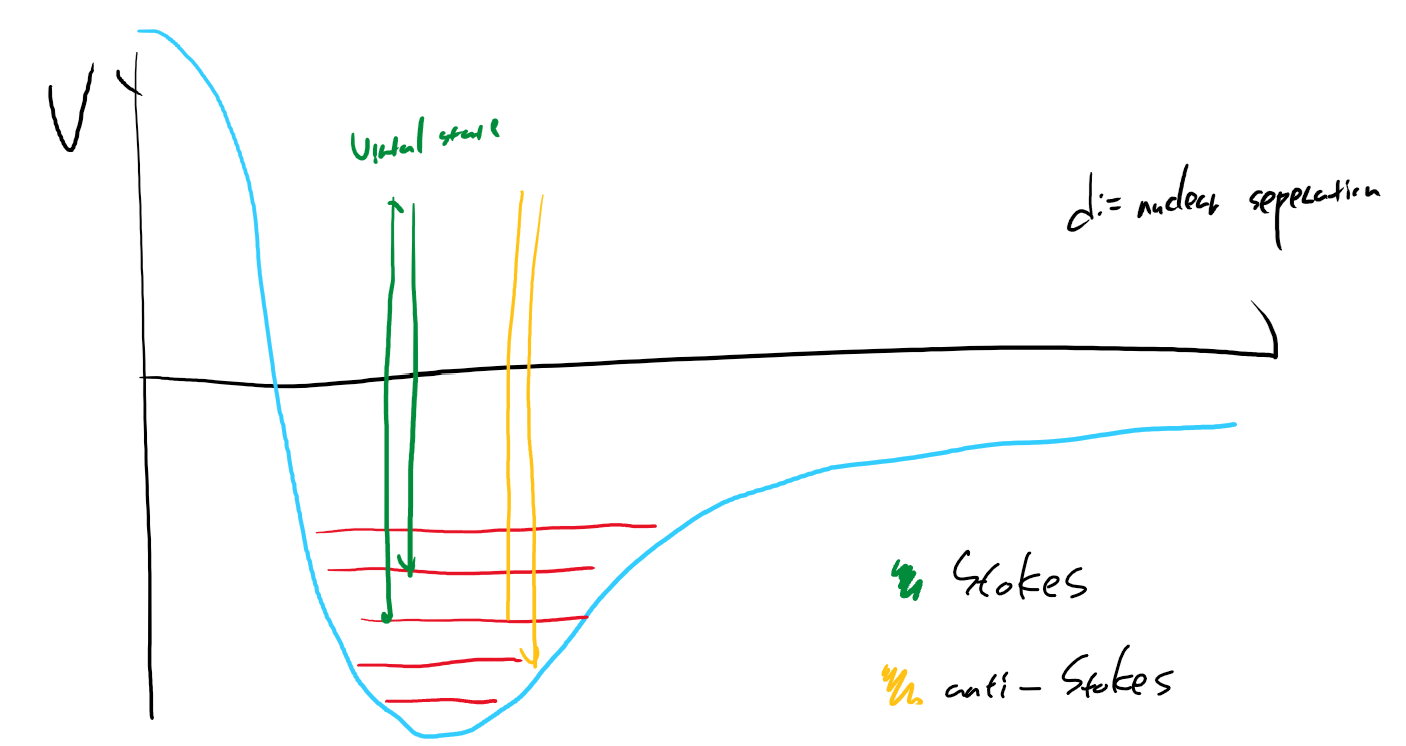
\includegraphics[width=0.8\textwidth]{EnergyLevels.png} % Replace 'figure.jpg' with your image file
    \caption{Raman Shifting in an Iodine molecule}
    \label{fig:example}
\end{figure}

We continue our discourse of vibrational peaks in an Iodine molecue. 
The potential of a two atom system diverges to infinity around $r = 0$ 
and asymptotes to zero at $r \rightarrow \infty$. In between the 
two limits exists a well. At the global minimum of the potential well, 
Taylor series approximations reveal the well to be approximately a 
simple harmonic oscillator. Let $\omega$ be the resonant frequency 
of the approximated potential. Then, 
\begin{align}
    E_n & = \ (\frac 1 2 + n) \hbar \omega \ \ \ (n \ = \ 0, 1, 2, \dots) \\
    \Delta E & = \ \hbar \omega
\end{align}

\begin{question}
    What is the approximated "spring constant" at the bottom of the well?
\end{question}
\begin{proof}[Solution]
    The frequency of the oscillator is related to the spring constant. 
    \begin{align}
        \omega \ = \ \frac{\Delta E} \hbar \ = \sqrt{\frac k \mu}
    \end{align}
    Instead of mass, we use the reduced mass of the Iodine atom, 
    $\mu = m_I/2$. After algebraic manipulations, we deduce the following. 
    \begin{align}
        k \ = \ \frac {m_I} 2 \left(
            \frac {\Delta E}{\hbar}
        \right)^2
    \end{align}
\end{proof}

As the vibrational energy of the molecule increases, the well width of 
the approximated SHO increases too. The increase in well width leads 
to a smaller spring constant. The square root of the spring constant 
is proportional to the frequency, which is proportional to the energy 
difference between two consecutive vibrational modes. Therefore, around 
the top of the well where the well width approaches infinity, the spacings 
between the vibrational modes vanish. 


\section{Data and Analysis}
Plesae plot 
\begin{enumerate}
\item (week 1) Intensity vs wavelength/vibrational spacing for Benzene and water  
\item (week 2) Plot vibrational spacing (in $cm^-1$) vs vibrational quantum number. 
\end{enumerate}

\section{Frank-Condon factors and Overlap Integrals}

\begin{question}
Explain the observed 'long vibrational progression' of a single vibrational level
\end{question}


This part refers to the last problem in the lab handout. Please check glow for details. 

\end{document}
